\chapter{Resultados}

\section{Descubrimiento en GSE78220}

El análisis principal se realizó en GSE78220 (25 muestras, tumor, RNA-seq, anti-PD-1). Tras verificar que los datos están en escala FPKM lineal, se aplicó la transformación $\log_2(\text{FPKM}+1)$ y se realizó un filtrado explícito de baja expresión: se eliminaron los genes con FPKM $< 1$ en al menos 5 muestras (20\,\% del total), lo que redujo el transcriptoma de 25.268 genes originales a \textbf{14.549 genes testados} (Tabla~\ref{tab:qc_gse78220}). No se detectaron genes significativos tras corrección FDR, resultado esperable por el tamaño muestral. Se identificaron \textbf{539 genes nominales} ($p < 0{,}05$, $|logFC| \geq 0{,}5$) como candidatos exploratorios.

\begin{table}[H]
\centering
\caption{Control de calidad y filtrado en GSE78220.}
\label{tab:qc_gse78220}
\begin{tabularx}{\textwidth}{l r}
\toprule
Paso de filtrado & Genes \\
\midrule
Genes/filas originales & 25.268 \\
Retirados por varianza cero & 2.663 \\
Retirados por baja expresión (FPKM $< 1$ en $<$5 muestras) & 10.719 \\
\textbf{Genes retenidos para DEA} & \textbf{14.549} \\
\bottomrule
\end{tabularx}
\end{table}

El análisis de control de calidad incluyó un boxplot de distribuciones de expresión por muestra y un PCA coloreado por respuesta. Las distribuciones son homogéneas entre muestras y el PCA muestra cierta separación entre respondedores y no respondedores en PC1, aunque con solapamiento, coherente con la señal débil esperable dado el tamaño muestral.

\begin{table}[H]
\centering
\caption{Resumen del análisis de descubrimiento en GSE78220.}
\label{tab:discovery_gse78220}
\begin{tabularx}{\textwidth}{l l X}
\toprule
Resultado & Valor & Interpretación \\
\midrule
Muestras & 25 & Tamaño muestral reducido; análisis exploratorio. \\
Genes testados (tras QC) & 14.549 & Transcriptoma filtrado por FPKM y varianza. \\
Genes FDR $< 0{,}05$ & 0 & Compatible con baja potencia ($n=25$). \\
Genes nominales & 539 & Candidatos exploratorios para validación. \\
LOOCV — top 5 genes & AUC\,=\,0{,}853 & Señal exploratoria; no rendimiento clínico validado. \\
LOOCV — top 10 genes & AUC\,=\,0{,}686 & Disminuye al aumentar genes; patrón esperable. \\
\bottomrule
\end{tabularx}
\end{table}

El modelo predictivo exploratorio LOOCV alcanza su mejor rendimiento con una firma de \textbf{5 genes} (AUC $= 0{,}853$, exactitud $= 76\,\%$), lo que sugiere que un pequeño subconjunto de genes concentra la señal predictiva. Al aumentar el número de genes la AUC disminuye (top 10: AUC $= 0{,}686$; top 20: AUC $= 0{,}558$), patrón coherente con la inclusión de genes con menor señal real.

\subsection{Enriquecimiento funcional exploratorio en GSE78220}

Dado que ningún gen alcanzó significación estadística tras corrección FDR en el DEA principal (resultado esperable con $n=25$), el enriquecimiento funcional se realizó sobre los \textbf{539 genes nominales} ($p < 0{,}05$) como conjunto exploratorio. La ORA GO-BP (umbral de significación $p_{\text{adj}} < 0{,}10$) debe interpretarse en este contexto: no refleja genes validados estadísticamente, sino tendencias biológicas observadas en la muestra de descubrimiento. Se separaron genes con mayor expresión en respondedores (\textit{up in R}) y en no respondedores (\textit{down in R}). Los resultados más relevantes se presentan en la Tabla~\ref{tab:ora_gse78220}.

\begin{table}[H]
\centering
\caption{Principales términos GO-BP enriquecidos en el análisis de descubrimiento exploratorio (GSE78220). \textit{Down in R}: más expresados en no respondedores; \textit{Up in R}: más expresados en respondedores.}
\label{tab:ora_gse78220}
\begin{tabularx}{\textwidth}{l l r r}
\toprule
Dirección & Término GO-BP & FDR & $n$ genes \\
\midrule
\textit{Down in R} & Extracellular matrix organization & $1{,}2\times10^{-22}$ & 44 \\
\textit{Down in R} & Angiogenesis & $9{,}1\times10^{-12}$ & 43 \\
\textit{Down in R} & Collagen fibril organization & $2{,}8\times10^{-9}$ & 15 \\
\textit{Down in R} & VEGFR signaling pathway & $8{,}6\times10^{-8}$ & 16 \\
\textit{Down in R} & Connective tissue development & $1{,}6\times10^{-6}$ & 23 \\
\midrule
\textit{Up in R} & Amino acid catabolic process & 0{,}033 & 8 \\
\textit{Up in R} & Respiratory electron transport chain & 0{,}033 & 8 \\
\textit{Up in R} & Cytoplasmic translation & 0{,}033 & 10 \\
\bottomrule
\end{tabularx}
\end{table}

Los genes más altos en no respondedores están fuertemente enriquecidos en remodelación de la matriz extracelular (MEC), angiogénesis y activación estromal (colágenos, metaloproteasas, PDGFR, VEGFC), lo que apunta a un fenotipo mesenquimal-estromal asociado a resistencia a inmunoterapia. Los genes con mayor expresión en respondedores se asocian a metabolismo mitocondrial y síntesis proteica, coherentes con un microambiente tumoral metabólicamente activo e inmunológicamente competente.

\section{Validación tumoral}

La validación de los genes candidatos en las cohortes tumorales NanoString mostró solapamiento limitado, esperable por las diferencias de plataforma. En GSE215868 (105 muestras, NanoString, anti-PD-1), \textbf{6 de los top 50 genes} de descubrimiento estaban presentes en el panel y el 66{,}7\,\% mantuvo la misma dirección de efecto; la AUC de la firma fue de 0{,}547. En GSE211645 (40 muestras, NanoString, anti-CTLA-4), únicamente 1 gen solapó, por lo que se interpreta como generalización exploratoria a otro checkpoint y no como validación directa.

\begin{table}[H]
\centering
\caption{Resumen de la validación tumoral. La firma se calculó con los top 100 genes de GSE78220 presentes en cada panel.}
\label{tab:validacion_tumoral}
\begin{tabularx}{\textwidth}{l r r r r X}
\toprule
Cohorte & $n$ & NR/R & Solapam. top 50 & Dir. concord. & AUC \\
\midrule
GSE215868 & 105 & 59/45 & 6 genes & 66{,}7\,\% & 0{,}547 \\
GSE211645 & 40 & 28/12 & 1 gen & --- & 0{,}390 \\
\bottomrule
\end{tabularx}
\end{table}

\section{Sensibilidad en sangre}

La firma tumoral anti-PD-1 no mostró señal predictiva en sangre periférica. GSE91061 (51 muestras, RNA-seq, varios ICI) alcanzó AUC $= 0{,}474$ con 19 genes de la firma disponibles. GSE94873 (360 muestras, NanoString, anti-CTLA-4) alcanzó AUC $= 0{,}475$ con \textbf{solo 4 genes de firma con solapamiento} en el panel de 162 sondas; este resultado debe interpretarse con extrema prudencia: con únicamente 4 genes, el score de firma no puede considerarse una evaluación representativa de la firma original y el análisis tiene valor exclusivamente como sensibilidad exploratoria, no como validación formal. Ambos resultados son coherentes con la distancia biológica (tumor vs.\ sangre) y técnica (plataforma, checkpoint) entre las cohortes.

\begin{table}[H]
\centering
\caption{Análisis de sensibilidad en sangre. NR: no respondedores; R: respondedores.}
\label{tab:sensibilidad_sangre}
\begin{tabularx}{\textwidth}{l r r r r X}
\toprule
Cohorte & $n$ & NR/R & Genes firma & AUC & Distancia \\
\midrule
GSE91061 & 51 & 39/10 & 19 & 0{,}474 & Tumor→sangre; multi-ICI \\
GSE94873 & 360 & 314/46 & 4 & 0{,}475 & Tumor→sangre; anti-CTLA-4; NanoString \\
\bottomrule
\end{tabularx}
\end{table}

\section{Consistencia integrada en genes comunes}

El análisis de consistencia en 200 genes comunes entre cohortes tumorales identificó 69 genes concordantes en las tres cohortes, 61 con efecto positivo y 8 con efecto negativo. La señal más coherente se relacionó con presentación antigénica por MHC-I y respuesta a IFN-gamma.

\begin{table}[H]
\centering
\caption{Consistencia multi-cohorte en genes comunes.}
\label{tab:consistencia}
\begin{tabularx}{\textwidth}{l l}
\toprule
Resultado & Valor \\
\midrule
Genes comunes evaluados & 200 \\
Genes up en las tres cohortes & 61 \\
Genes down en las tres cohortes & 8 \\
Genes discordantes & 131 \\
Genes destacados & HLA-A/B/C/E/F, PSMB8, IFNGR1, STAT2, SLAMF7, ICAM1 \\
\bottomrule
\end{tabularx}
\end{table}

\section{Bloque pronóstico TCGA-SKCM}

El bloque pronóstico se basa en TCGA-SKCM \cite{TCGA}, cohorte de referencia en melanoma cutáneo. Su objetivo es identificar variables clínicas y transcriptómicas asociadas a la supervivencia global, de forma independiente al bloque predictivo. TCGA no contiene información homogénea de tratamiento con inmunoterapia ni respuesta clínica binaria, por lo que su análisis se centra en el pronóstico.

\subsection{Descripción de la cohorte}

La descarga mediante TCGAbiolinks proporcionó datos clínicos de 470 pacientes con 90 variables. Las variables de supervivencia se construyeron del siguiente modo: \texttt{OS\_event} = 1 si \texttt{vital\_status = Dead}, 0 si \texttt{vital\_status = Alive}; \texttt{OS\_time} se obtuvo de \texttt{days\_to\_death} en pacientes fallecidos y de \texttt{days\_to\_last\_follow\_up} en los censurados. Tras excluir casos con tiempo negativo o variables ausentes, el conjunto de datos válido para el análisis de supervivencia quedó integrado por 470 pacientes.

\subsection{Curvas de Kaplan-Meier}

Se generaron curvas de Kaplan-Meier globales y por subgrupos. La curva de supervivencia global muestra un descenso progresivo a lo largo del seguimiento, con una mediana de supervivencia estimada en torno a los 2--3 años (Figura~\ref{fig:km_global}).

\begin{figure}[H]
\centering
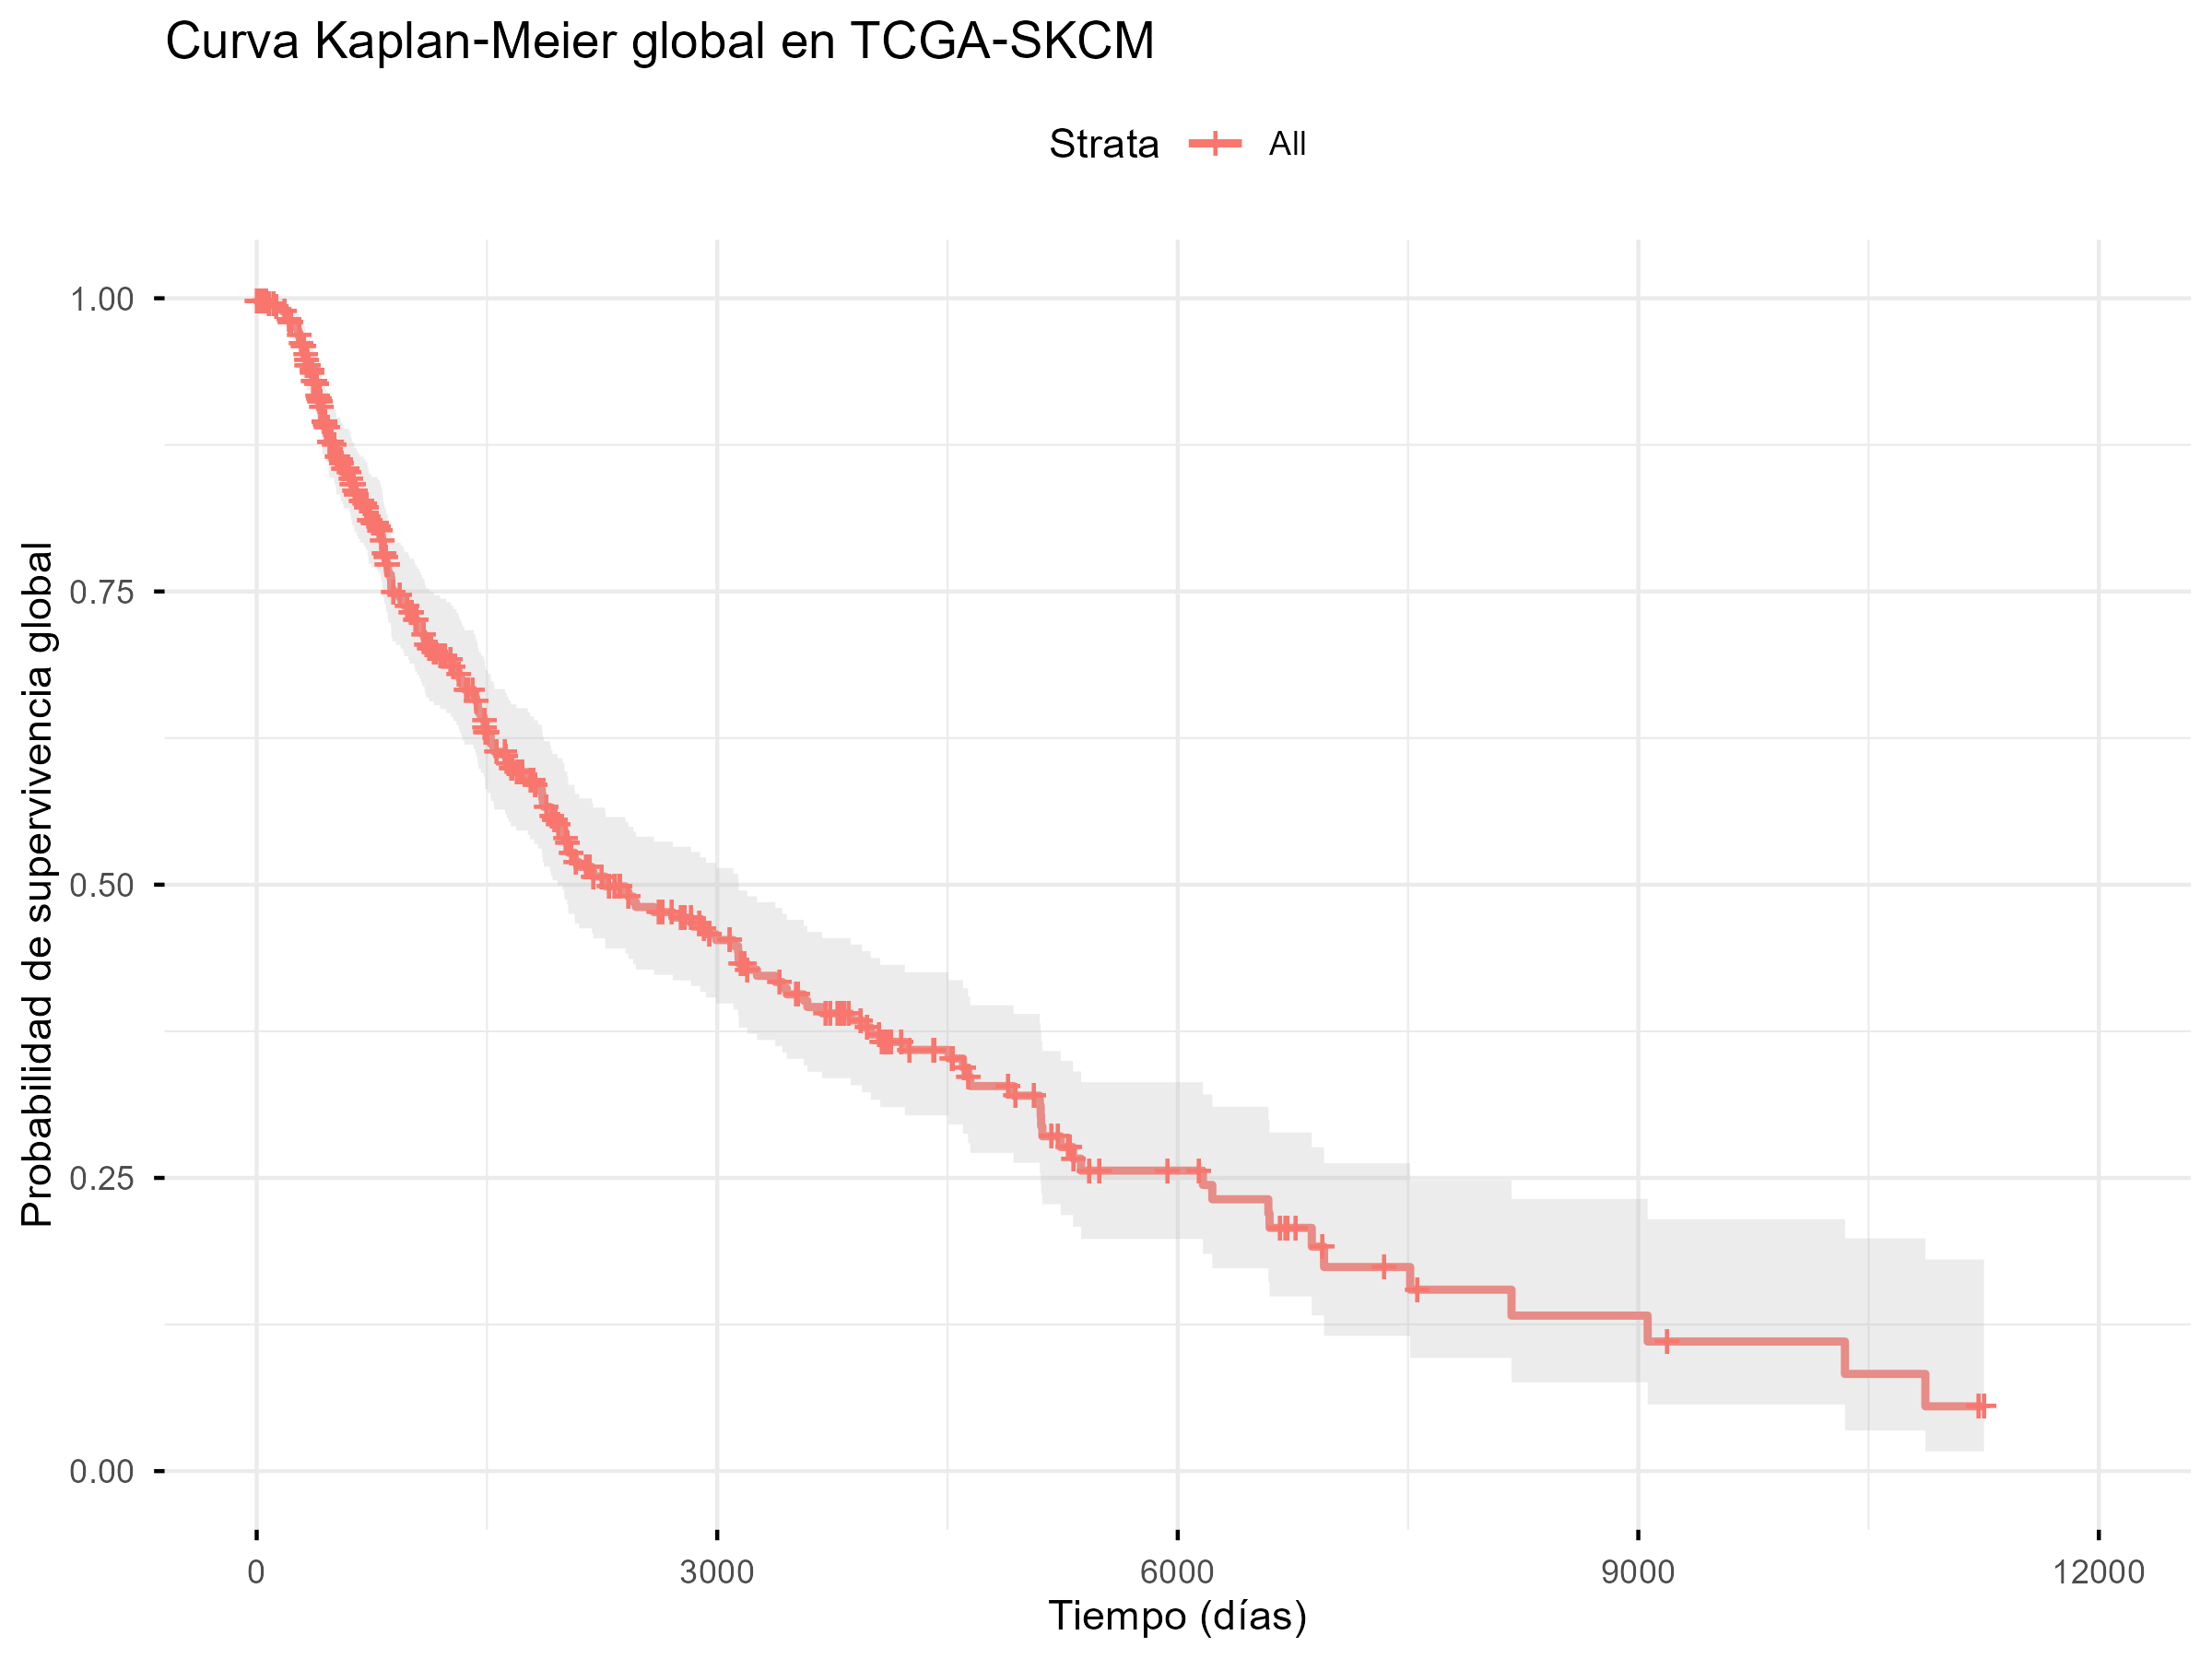
\includegraphics[width=0.85\textwidth]{figures/km_global_plot}
\caption{Curva de Kaplan-Meier de supervivencia global en TCGA-SKCM (N\,=\,470).}
\label{fig:km_global}
\end{figure}

El análisis por sexo no mostró diferencias estadísticamente significativas mediante el test log-rank, resultado coherente con los modelos Cox (Figura~\ref{fig:km_sexo_estadio}). Por el contrario, el análisis por estadio AJCC evidenció una separación progresiva de las curvas conforme aumenta el estadio, con peor pronóstico en estadio IV, confirmando la validez del sistema de estadificación como marcador pronóstico en esta cohorte.

\begin{figure}[H]
\centering
\begin{minipage}[t]{0.48\textwidth}
  \centering
  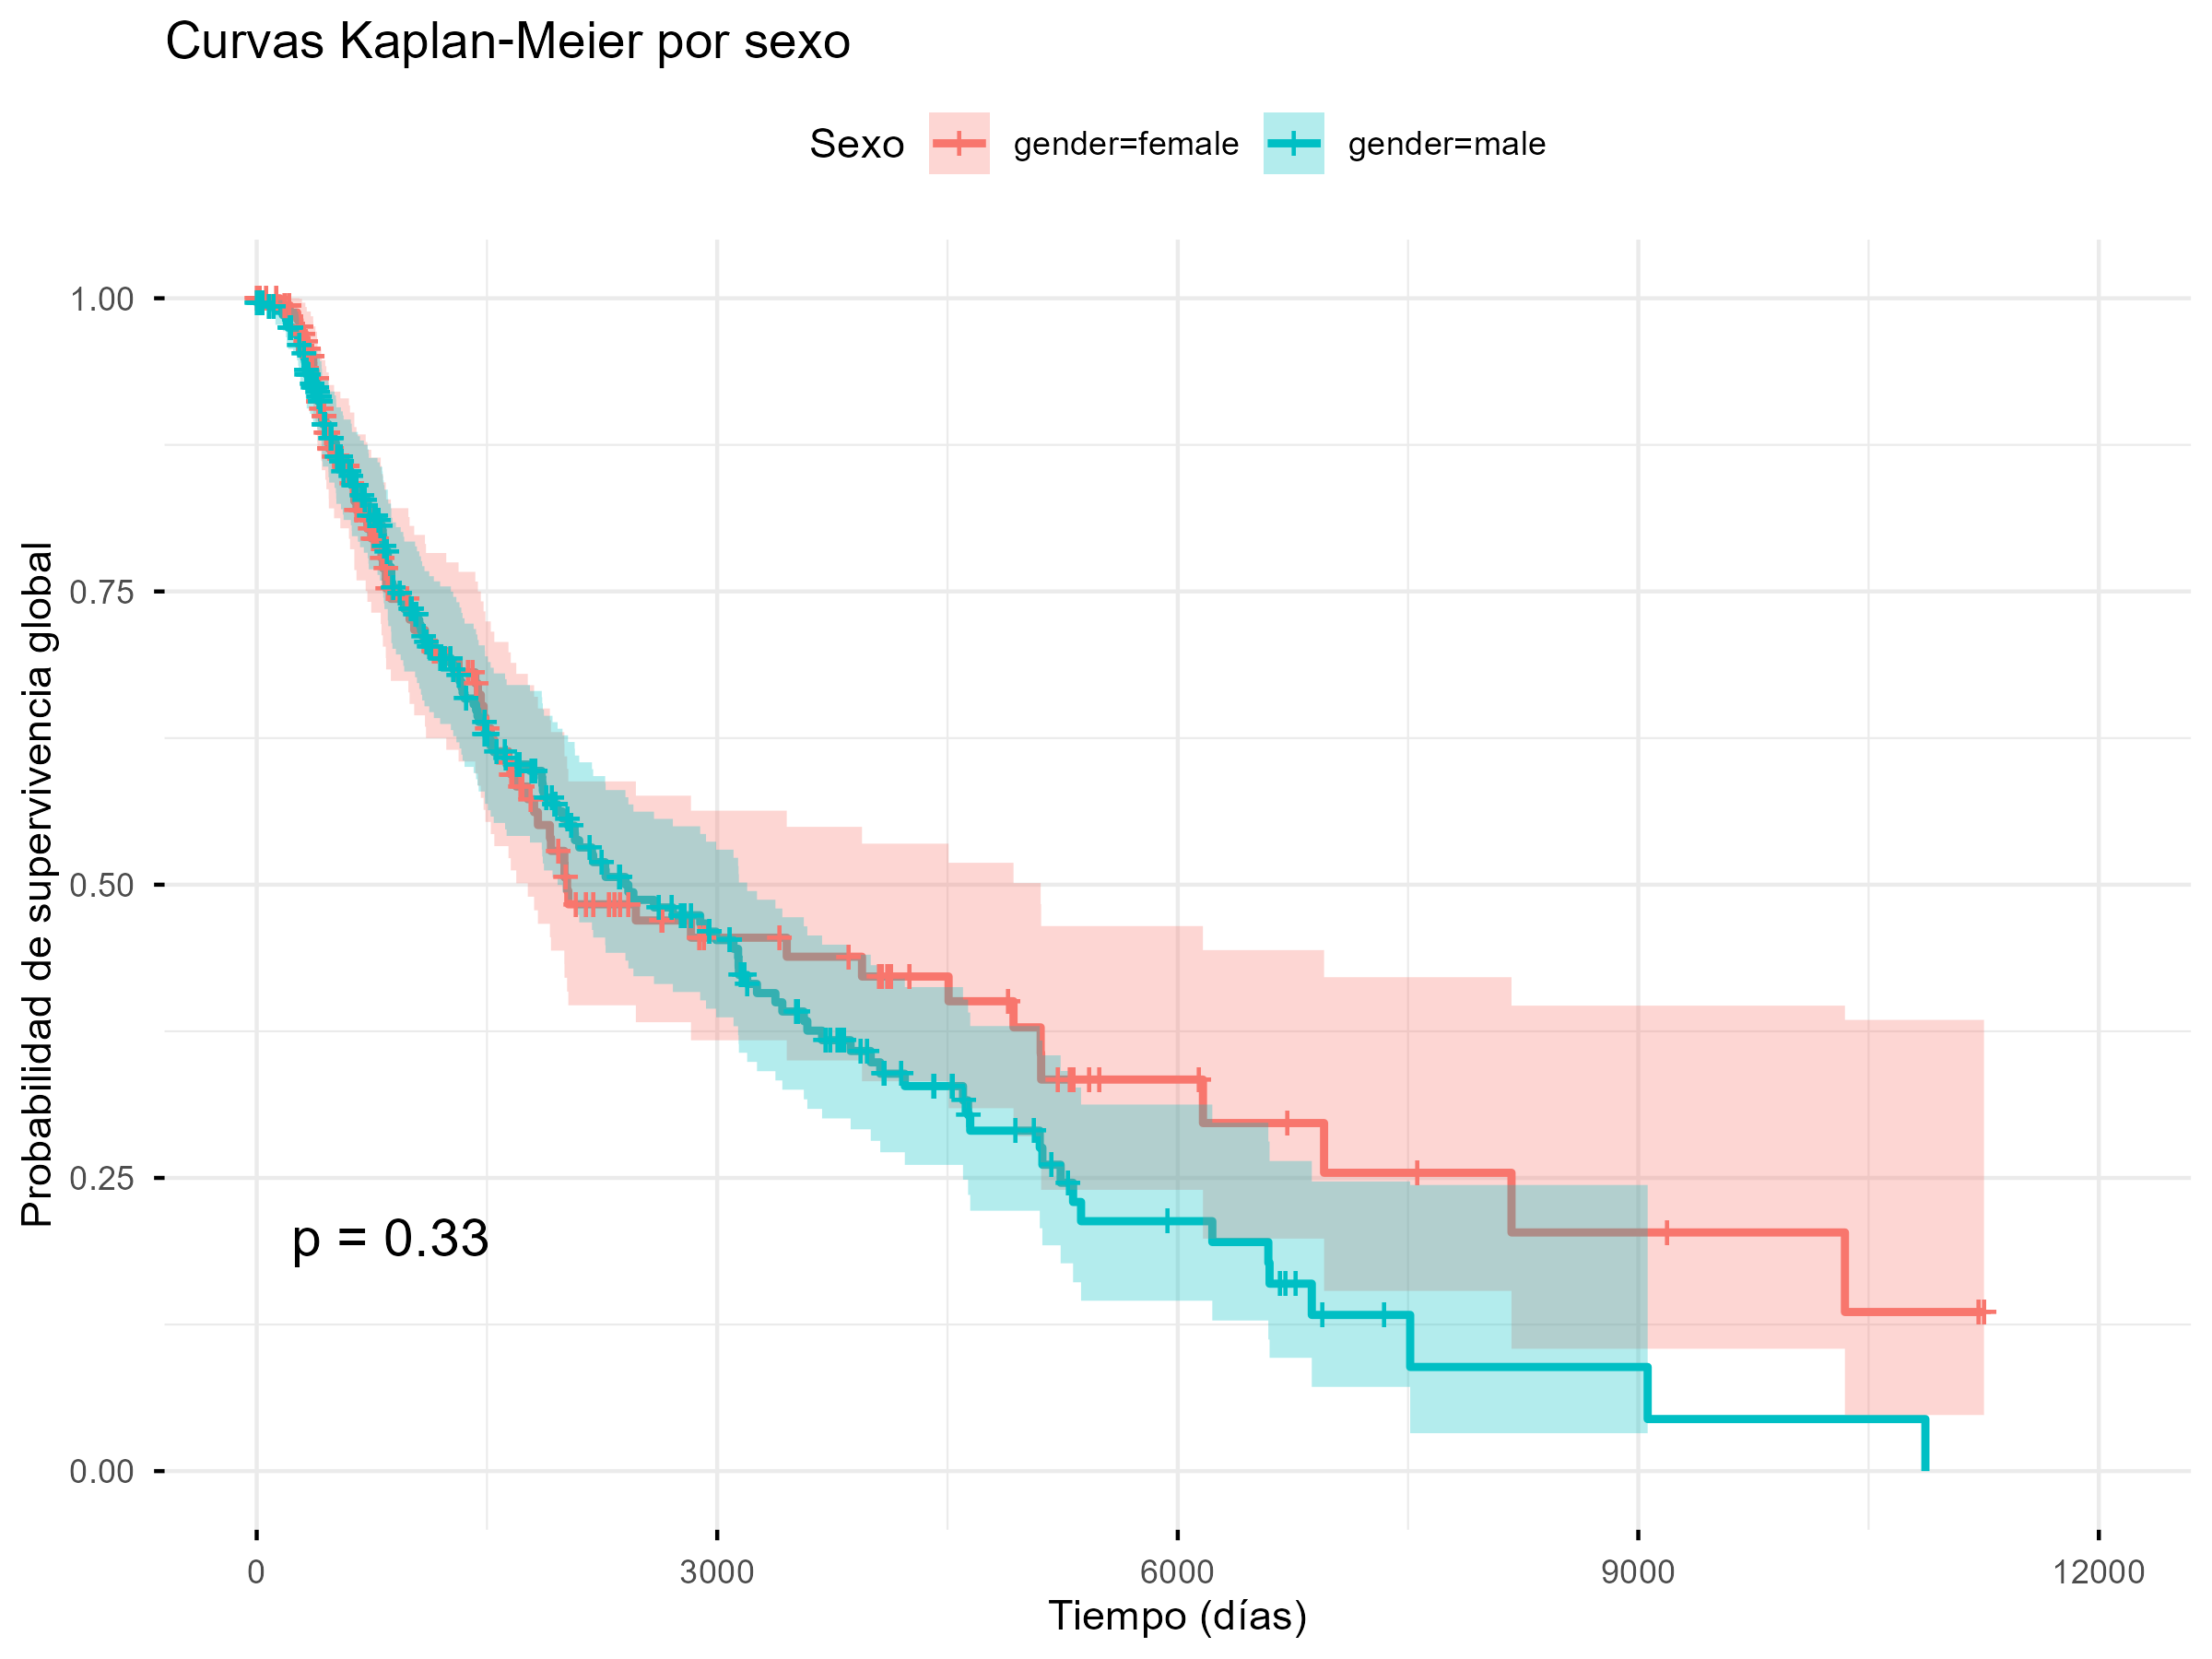
\includegraphics[width=\textwidth]{figures/km_gender_plot}
\end{minipage}
\hfill
\begin{minipage}[t]{0.48\textwidth}
  \centering
  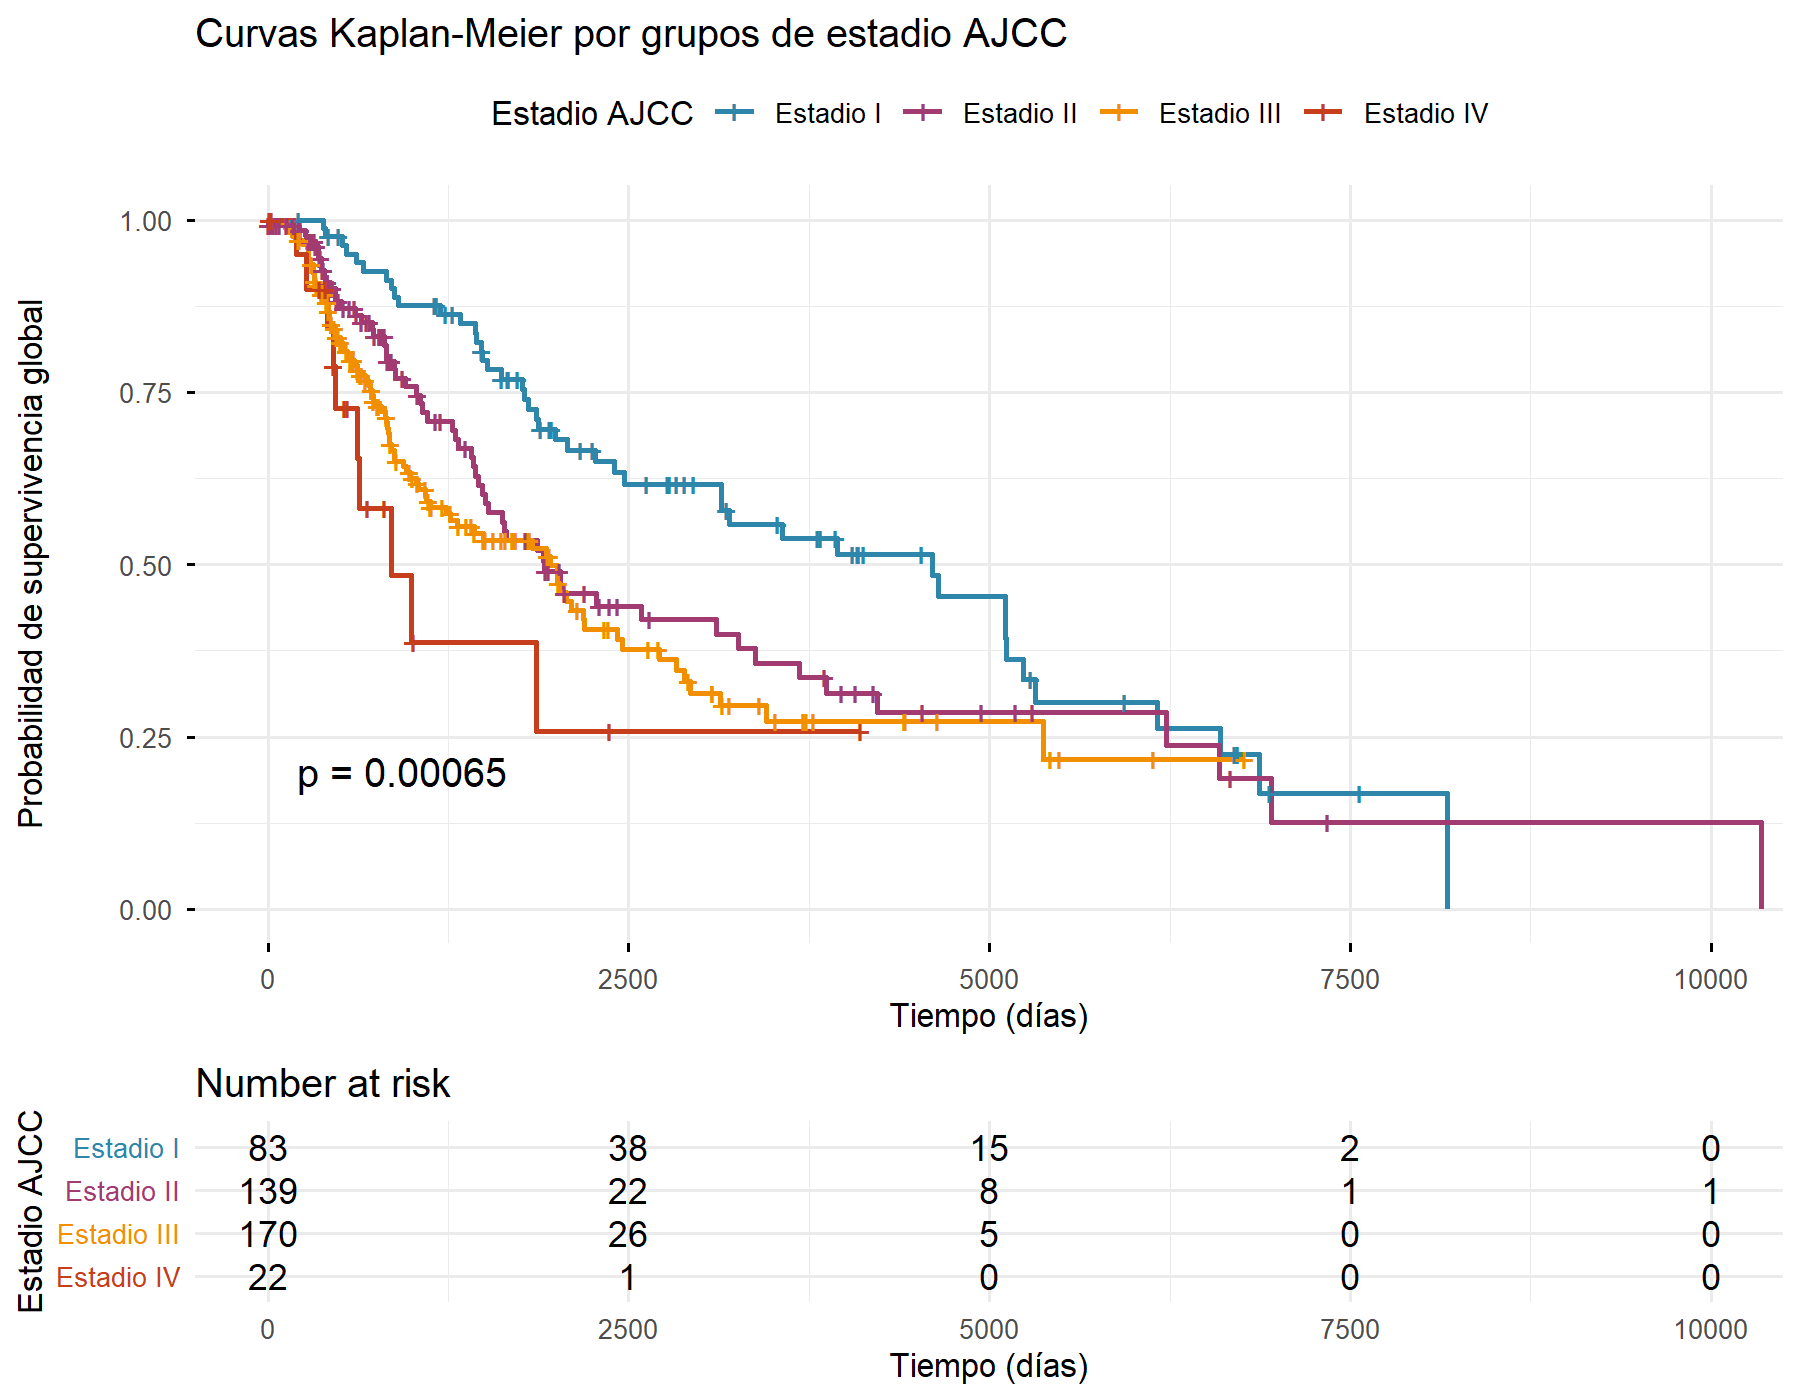
\includegraphics[width=\textwidth]{figures/km_stage_group_plot}
\end{minipage}
\caption{Izquierda: curva de Kaplan-Meier por sexo (test log-rank, p\,=\,NS). Derecha: curva de Kaplan-Meier por estadio AJCC agrupado (I--II vs.\ III--IV).}
\label{fig:km_sexo_estadio}
\end{figure}

\subsection{Factores pronósticos clínicos: modelo Cox univariante}

Se ajustaron modelos de Cox univariantes para edad, sexo y estadio AJCC (simplificado en cuatro grupos: I, II, III y IV). Los resultados se resumen en la Tabla~\ref{tab:cox_univariante_tcga}.

\begin{table}[H]
\centering
\caption{Resultados del modelo de Cox univariante en TCGA-SKCM. HR: hazard ratio; IC~95\,\%: intervalo de confianza al 95\,\%; p: p-valor. Estadio de referencia: estadio I.}
\label{tab:cox_univariante_tcga}
\begin{tabularx}{\textwidth}{l r r r}
\toprule
Variable & HR & IC 95\,\% & $p$ \\
\midrule
Edad (años) & 1,021 & (1,011--1,031) & $<0{,}001$ \\
Sexo (masculino vs.\ femenino) & 1,006 & (0,747--1,354) & 0,969 \\
Estadio II vs.\ I & 1,518 & (1,023--2,251) & 0,038 \\
Estadio III vs.\ I & 1,952 & (1,344--2,834) & $<0{,}001$ \\
Estadio IV vs.\ I & 3,094 & (1,540--6,215) & 0,002 \\
\bottomrule
\end{tabularx}
\end{table}

La edad se asocia de forma significativa con peor supervivencia: por cada año adicional de edad, el riesgo de muerte aumenta en un 2,1\,\% (HR = 1{,}021; IC~95\,\%: 1{,}011--1{,}031; $p < 0{,}001$). El sexo masculino no presenta asociación significativa con la supervivencia (HR = 1{,}006; $p = 0{,}969$). El estadio IV se asocia a un riesgo de muerte tres veces superior respecto al estadio I (HR = 3{,}094; IC~95\,\%: 1{,}540--6{,}215; $p = 0{,}002$).

\subsection{Modelo de Cox multivariante}

El modelo de Cox multivariante incluyó simultáneamente edad, sexo y estadio. Los resultados se presentan en la Tabla~\ref{tab:cox_multivariante_tcga}.

\begin{table}[H]
\centering
\caption{Resultados del modelo de Cox multivariante en TCGA-SKCM. HR ajustado por las demás covariables del modelo. Estadio de referencia: estadio I.}
\label{tab:cox_multivariante_tcga}
\begin{tabularx}{\textwidth}{l r r r}
\toprule
Variable & HR ajustado & IC 95\,\% & $p$ \\
\midrule
Edad (años) & 1,020 & (1,010--1,031) & $<0{,}001$ \\
Sexo (masculino vs.\ femenino) & 1,007 & (0,747--1,357) & 0,963 \\
Estadio II vs.\ I & 1,265 & (0,843--1,898) & 0,257 \\
Estadio III vs.\ I & 1,819 & (1,248--2,652) & 0,002 \\
Estadio IV vs.\ I & 2,993 & (1,486--6,028) & 0,002 \\
\bottomrule
\end{tabularx}
\end{table}

El ajuste multivariante revela que la edad y los estadios III--IV mantienen su asociación independiente con la supervivencia. Destaca que el estadio II pierde significación estadística en el modelo multivariante (HR = 1{,}265; $p = 0{,}257$), lo que sugiere que su efecto aparente en el modelo univariante podría estar parcialmente mediado por la distribución de la edad entre estadios. El sexo no es un factor pronóstico independiente en esta cohorte (HR = 1{,}007; $p = 0{,}963$). La validación del supuesto de riesgos proporcionales se realizó mediante el test de Schoenfeld (función \texttt{cox.zph}). El forest plot del modelo multivariante se presenta en la Figura~\ref{fig:forest_multi}.

\begin{figure}[H]
\centering
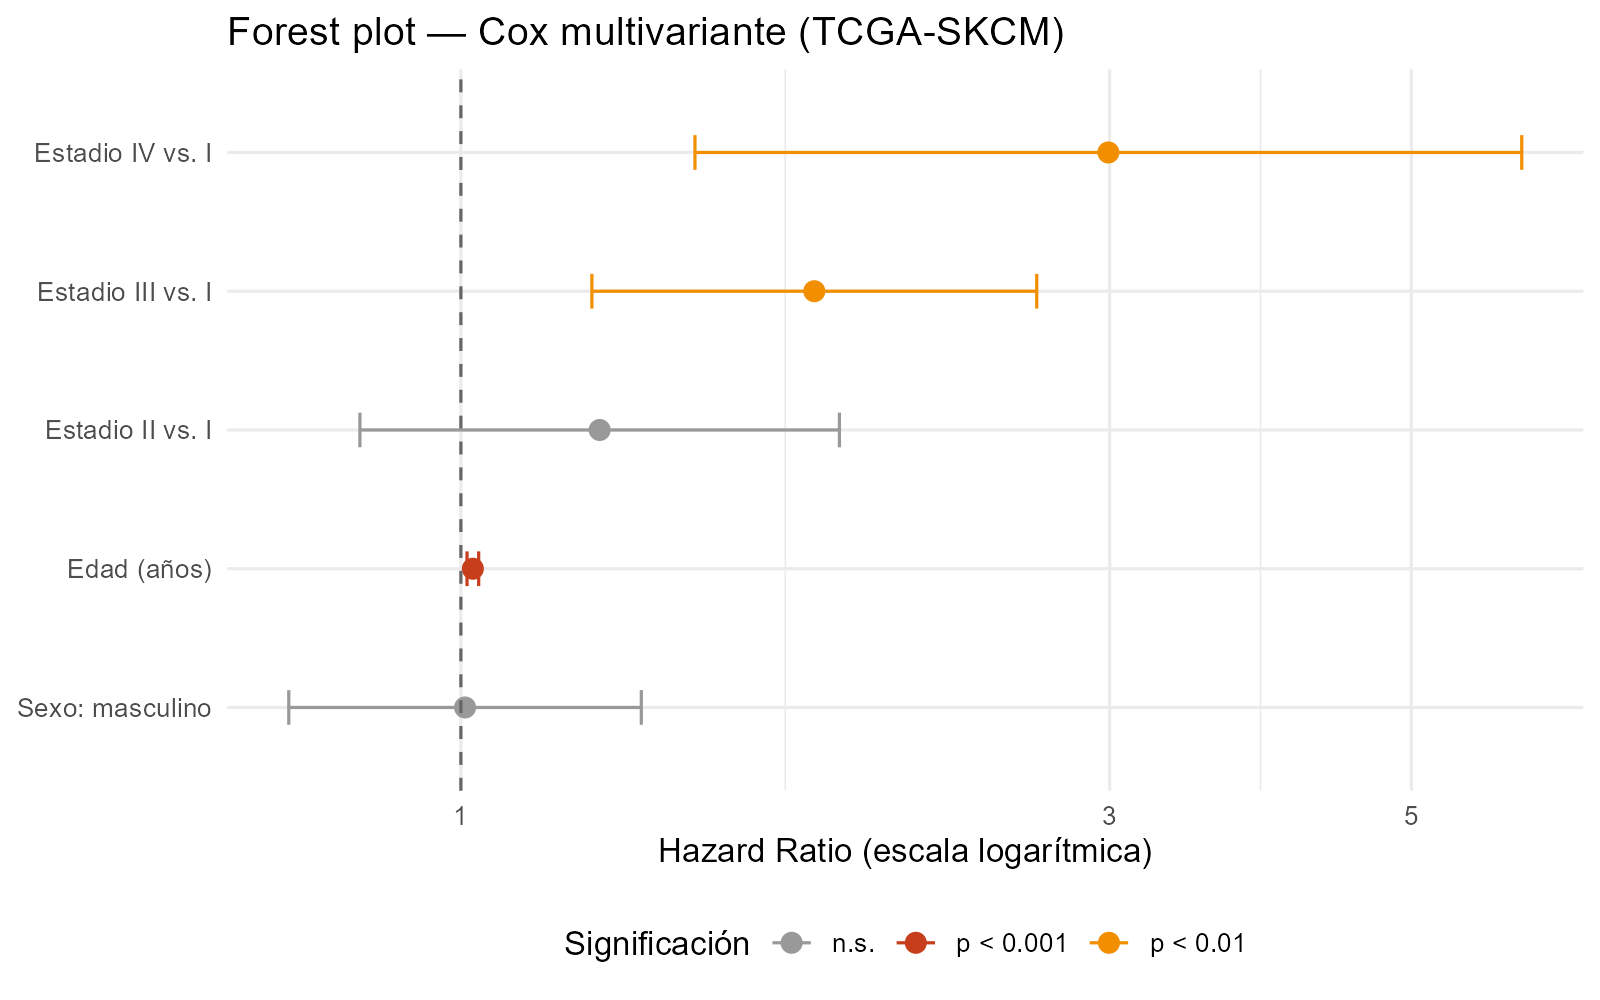
\includegraphics[width=0.80\textwidth]{figures/cox_multivariate_forest_plot}
\caption{Forest plot del modelo de Cox multivariante en TCGA-SKCM. Cada punto indica el HR puntual y las líneas horizontales el IC~95\,\%. La línea vertical discontinua marca HR\,=\,1 (ausencia de efecto). Escala logarítmica en el eje horizontal.}
\label{fig:forest_multi}
\end{figure}

\subsection{Screening transcriptómico: Cox gen a gen}

Tras la normalización de los datos de expresión RNA-seq (log-CPM) y la selección de los genes más variables (script \texttt{08\_tcga\_skcm\_transcriptomics\_corregido.Rmd}), se construyó un \textit{master dataset} que integra las variables clínicas de supervivencia con la matriz de expresión. El screening transcriptómico consistió en ajustar un modelo de Cox univariante por gen sobre los 5.002 genes más variables de la cohorte, empleando como variable independiente la expresión de cada gen (escala log-CPM).

Los resultados del screening se resumen a continuación:

\begin{itemize}
  \item Genes testados: 5.002
  \item Genes con $p < 0{,}05$ (nominal): 1.951 (39,0\,\%)
  \item Genes con FDR $< 0{,}05$: 1.439 (28,8\,\%)
  \item Genes con FDR $< 0{,}01$: 944 (18,9\,\%)
\end{itemize}

El gen con menor FDR es \textit{GBP2} (HR = 0{,}776; $p = 4{,}15\times10^{-11}$; FDR = $2{,}08\times10^{-7}$). El patrón direccional de los 15 genes con menor FDR es predominantemente protector (12 de 15 con HR $< 1$), lo que indica que su alta expresión se asocia a mejor supervivencia. Este patrón es biológicamente coherente con un papel favorecedor del sistema inmune: la mayoría de los genes candidatos pertenecen a vías de señalización por interferón, activación de células NK y reclutamiento de linfocitos T citotóxicos.

Los diez genes con menor FDR, anotados a partir del identificador Ensembl mediante la API REST de Ensembl, se presentan en la Tabla~\ref{tab:top_genes_tcga}.

\begin{table}[H]
\centering
\caption{Diez genes con menor FDR en el screening Cox transcriptómico (TCGA-SKCM). HR calculado por modelo Cox univariante; FDR obtenido mediante ajuste Benjamini-Hochberg sobre 5.002 genes. HR $< 1$ indica efecto protector (alta expresión asociada a mayor supervivencia).}
\label{tab:top_genes_tcga}
\begin{tabularx}{\textwidth}{l r r X}
\toprule
Gen & HR & FDR & Función biológica \\
\midrule
\textit{GBP2}     & 0,776 & $2{,}1\times10^{-7}$ & Proteína de unión a guanilato inducida por IFN-$\gamma$ \\
\textit{GBP4}     & 0,834 & $1{,}1\times10^{-6}$ & Proteína de unión a guanilato inducida por IFN-$\gamma$ \\
\textit{IL15}     & 0,793 & $1{,}1\times10^{-6}$ & Interleucina 15; activación de células NK y CD8$^+$ \\
\textit{GIMAP2}   & 0,763 & $1{,}1\times10^{-6}$ & GTPasa IMAP; supervivencia de linfocitos \\
\textit{DDX60}    & 0,750 & $1{,}1\times10^{-6}$ & Helicasa innata; señalización por interferón antiviral \\
\textit{KLRD1}    & 0,823 & $1{,}4\times10^{-6}$ & CD94; receptor activador/inhibidor de células NK \\
\textit{CCL8}     & 0,827 & $1{,}4\times10^{-6}$ & Quimiocina MCP-2; reclutamiento de linfocitos T \\
\textit{GCNT1}    & 0,775 & $1{,}7\times10^{-6}$ & Glucosaminil-transferasa; glicosilación de glucolípidos \\
\textit{APOBEC3G} & 0,789 & $1{,}8\times10^{-6}$ & Editasa RNA/DNA; defensa antiviral innata \\
\textit{UBA7}     & 0,775 & $1{,}8\times10^{-6}$ & Enzima E1 de activación de ubiquitina; vía ISGilación \\
\bottomrule
\end{tabularx}
\end{table}

Los resultados completos de los 5.002 genes, rankeados por FDR, se han exportado al fichero \texttt{results/cox\_transcriptome\_results.csv}.

\subsection{Curvas de Kaplan-Meier para genes candidatos}

Para los 10 genes con menor FDR se generaron curvas de Kaplan-Meier estratificando las muestras en alta expresión (por encima de la mediana de la cohorte) vs.\ baja expresión (por debajo). En todos los casos la separación de curvas fue consistente con la dirección del efecto estimada por el modelo Cox: los pacientes con alta expresión de los genes protectores ($HR < 1$) presentaron mayor supervivencia. Esta coherencia interna entre el modelo paramétrico y las curvas no paramétricas refuerza la validez de los candidatos identificados.

Como ejemplo representativo, para \textit{GBP2} (el gen con menor FDR), la separación de curvas es marcada y el p-valor del test log-rank es altamente significativo, con el grupo de alta expresión presentando mejor pronóstico a todos los tiempos de seguimiento evaluados.

\subsection{Volcano plot del screening transcriptómico}

La Figura~\ref{fig:volcano_cox} presenta el volcano plot del screening Cox, donde el eje horizontal representa el logaritmo del hazard ratio [log(HR)], que indica la dirección del efecto, y el eje vertical representa $-\log_{10}(\text{FDR})$. Los genes en azul (log HR $< 0$) son protectores, los genes en rojo (log HR $> 0$) son de riesgo. El patrón global muestra una asimetría hacia el cuadrante protector, coherente con la hipótesis de que la activación inmune tumoral favorece la supervivencia en melanoma.

\begin{figure}[H]
\centering
\IfFileExists{figures/volcano_cox_transcriptomico.png}{%
  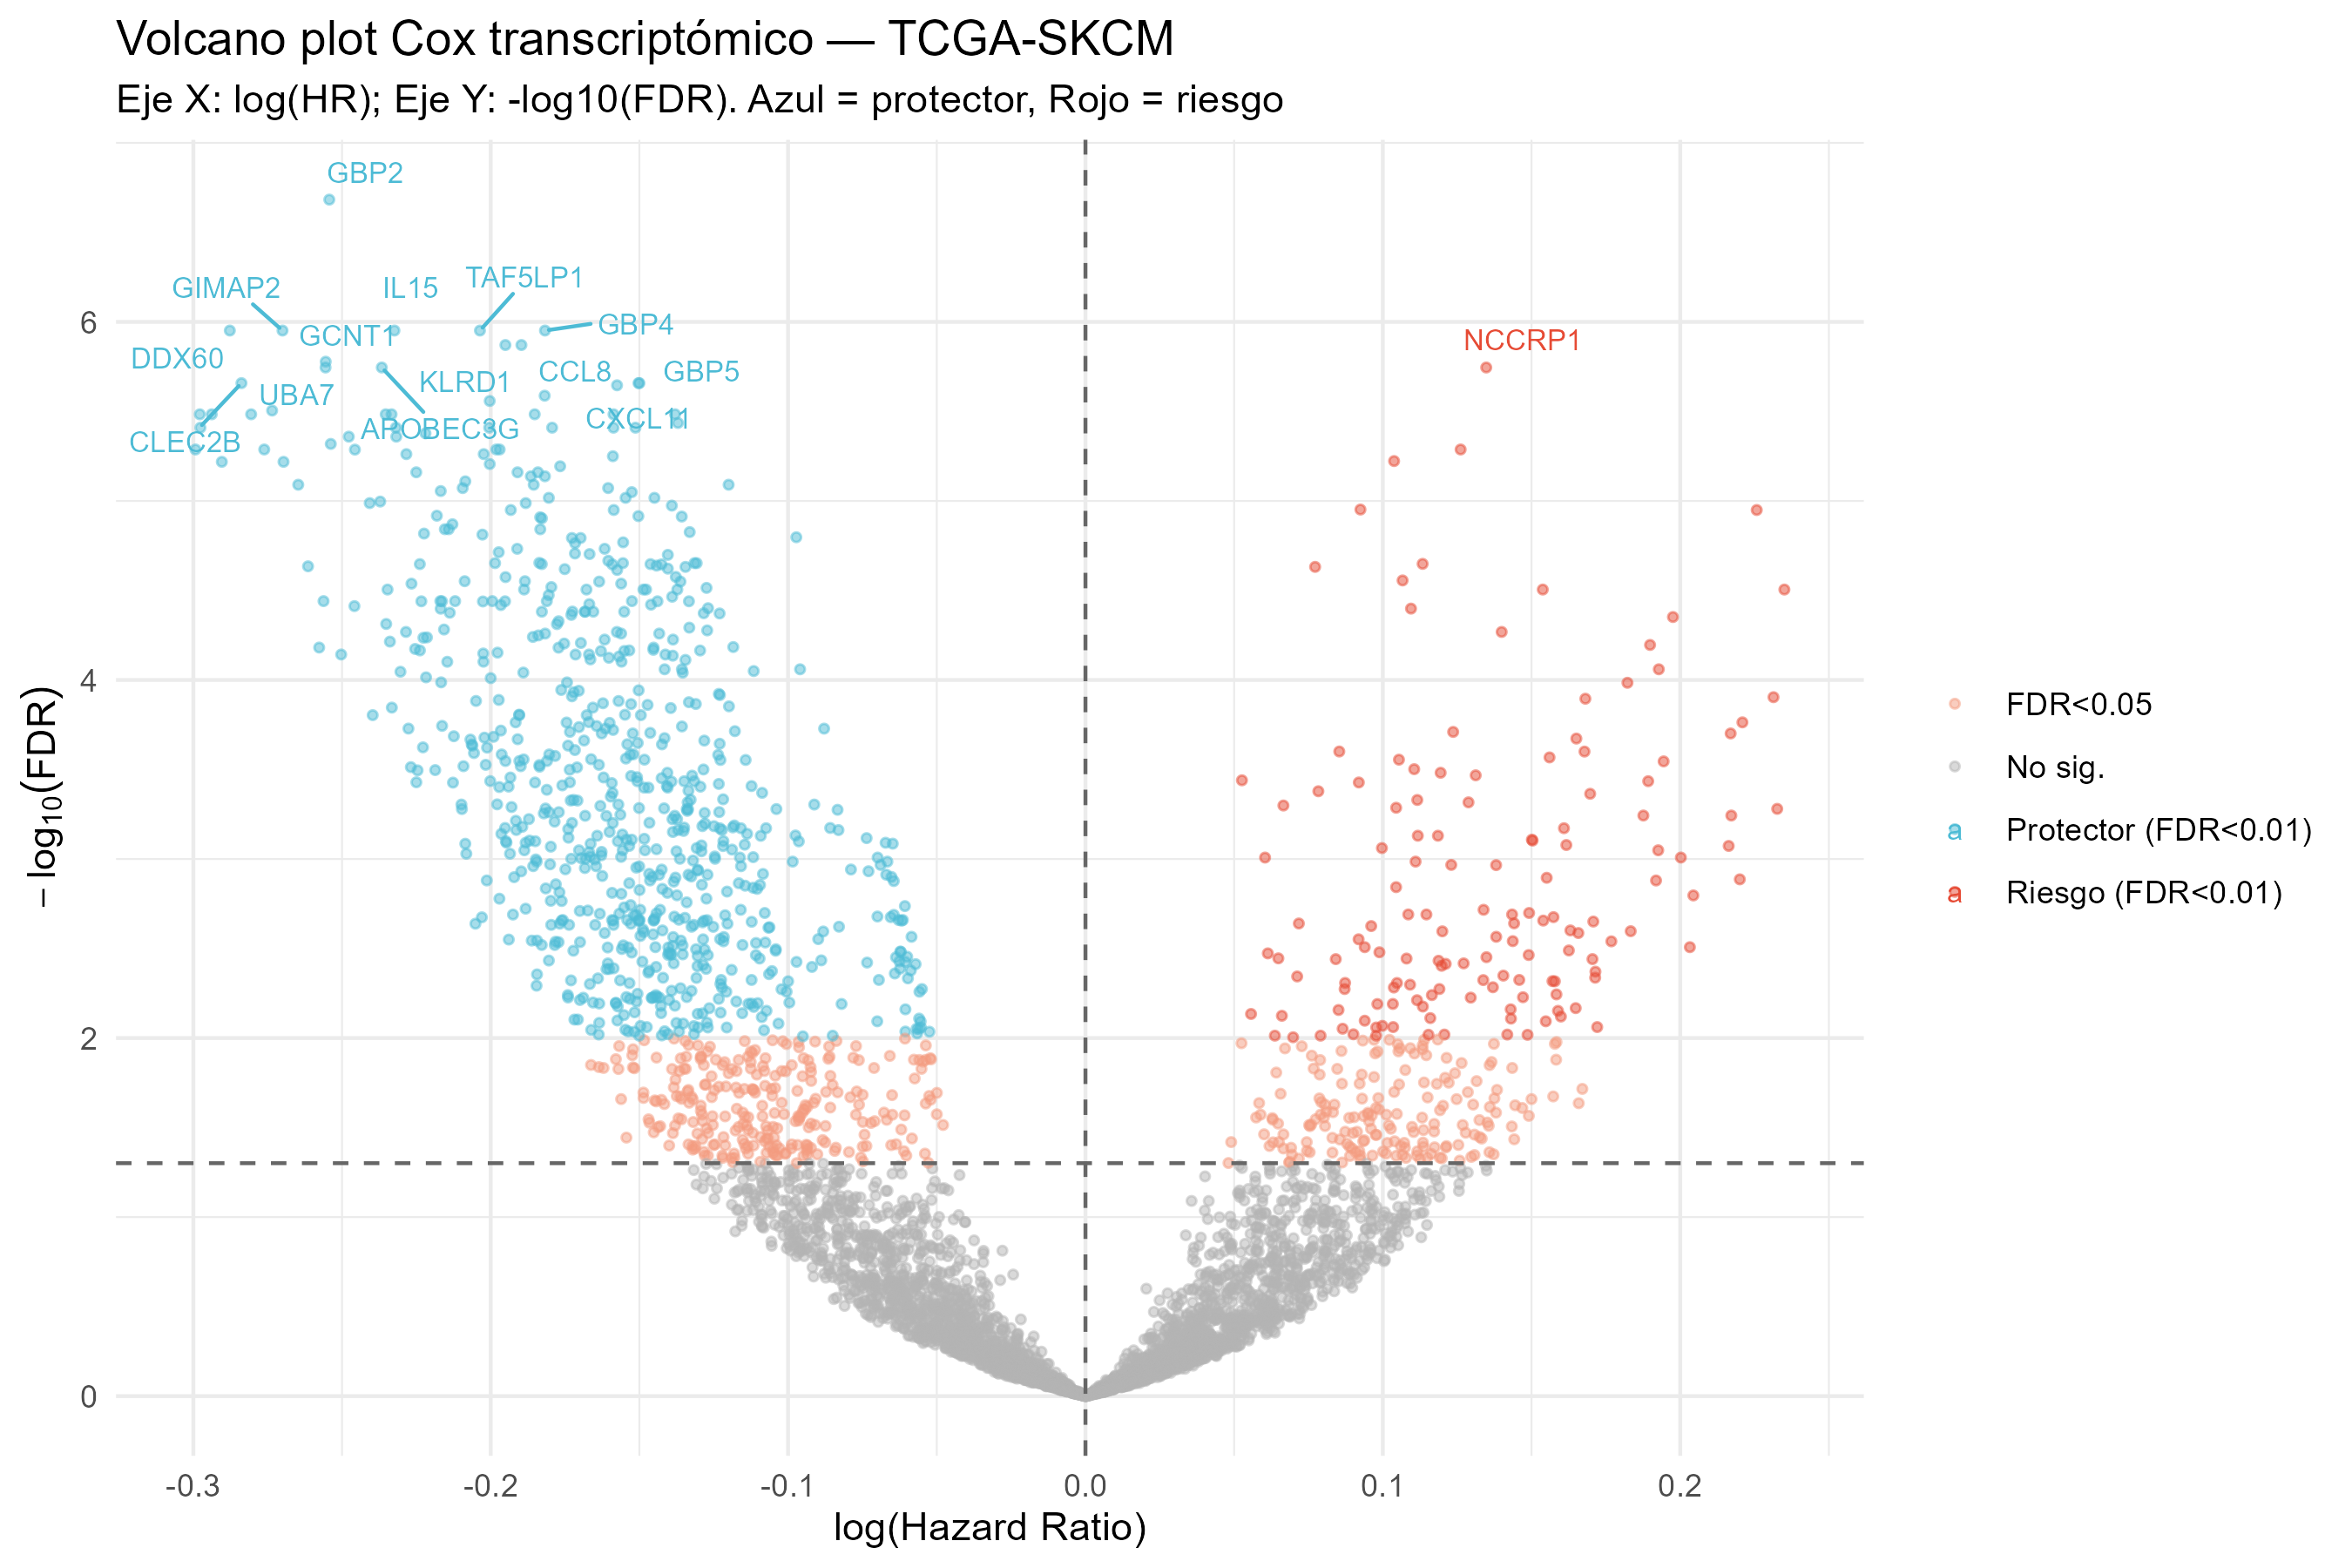
\includegraphics[width=0.90\textwidth]{figures/volcano_cox_transcriptomico}%
}{%
  \fbox{\begin{minipage}{0.85\textwidth}\centering\vspace{1.5cm}
  \textit{Figura pendiente: ejecutar \texttt{13\_tcga\_anotacion\_ora.Rmd} para generar\\
  \texttt{figures/volcano\_cox\_transcriptomico.png}}
  \vspace{1.5cm}\end{minipage}}%
}
\caption{Volcano plot del screening Cox gen a gen en TCGA-SKCM (5.002 genes). Eje X: log(HR); eje Y: $-\log_{10}$(FDR). Línea horizontal discontinua: FDR\,=\,0{,}05. Línea vertical discontinua: HR\,=\,1. Azul oscuro: genes protectores con FDR $< 0{,}01$; rojo: genes de riesgo con FDR $< 0{,}01$; naranja: FDR $< 0{,}05$; gris: no significativos. Etiquetados los 15 genes con menor FDR.}
\label{fig:volcano_cox}
\end{figure}

\subsection{Análisis de sobrerrepresentación funcional (ORA)}

Para interpretar biológicamente los genes asociados a la supervivencia, se realizó un análisis de sobrerrepresentación (ORA) sobre GO-BP mediante \texttt{clusterProfiler}, previa conversión de los identificadores Ensembl a Entrez ID con \texttt{org.Hs.eg.db}. Se analizaron por separado los genes protectores (FDR $< 0{,}05$, HR $< 1$) y los genes de riesgo (FDR $< 0{,}05$, HR $> 1$). Los resultados completos se presentarán tras la compilación del script \texttt{13\_tcga\_anotacion\_ora.Rmd}, cuyo código implementa fielmente la misma metodología aplicada en el análisis de RNA-seq de cáncer colorrectal (PEC2, análisis de datos ómicos).

Los resultados del ORA confirman la interpretación biológica anticipada. Los genes protectores (HR $< 1$, FDR $< 0{,}05$) están fuertemente enriquecidos en procesos de respuesta inmune adaptativa e innata: respuesta a IFN-$\gamma$, presentación antigénica, activación de células NK y señalización de linfocitos T citotóxicos (Figura~\ref{fig:ora_prot}). Los genes de riesgo (HR $> 1$, FDR $< 0{,}05$) muestran enriquecimiento en procesos de queratinización y diferenciación epitelial, coherentes con un perfil de menor infiltración inmune (Figura~\ref{fig:ora_risk}).

\begin{figure}[H]
\centering
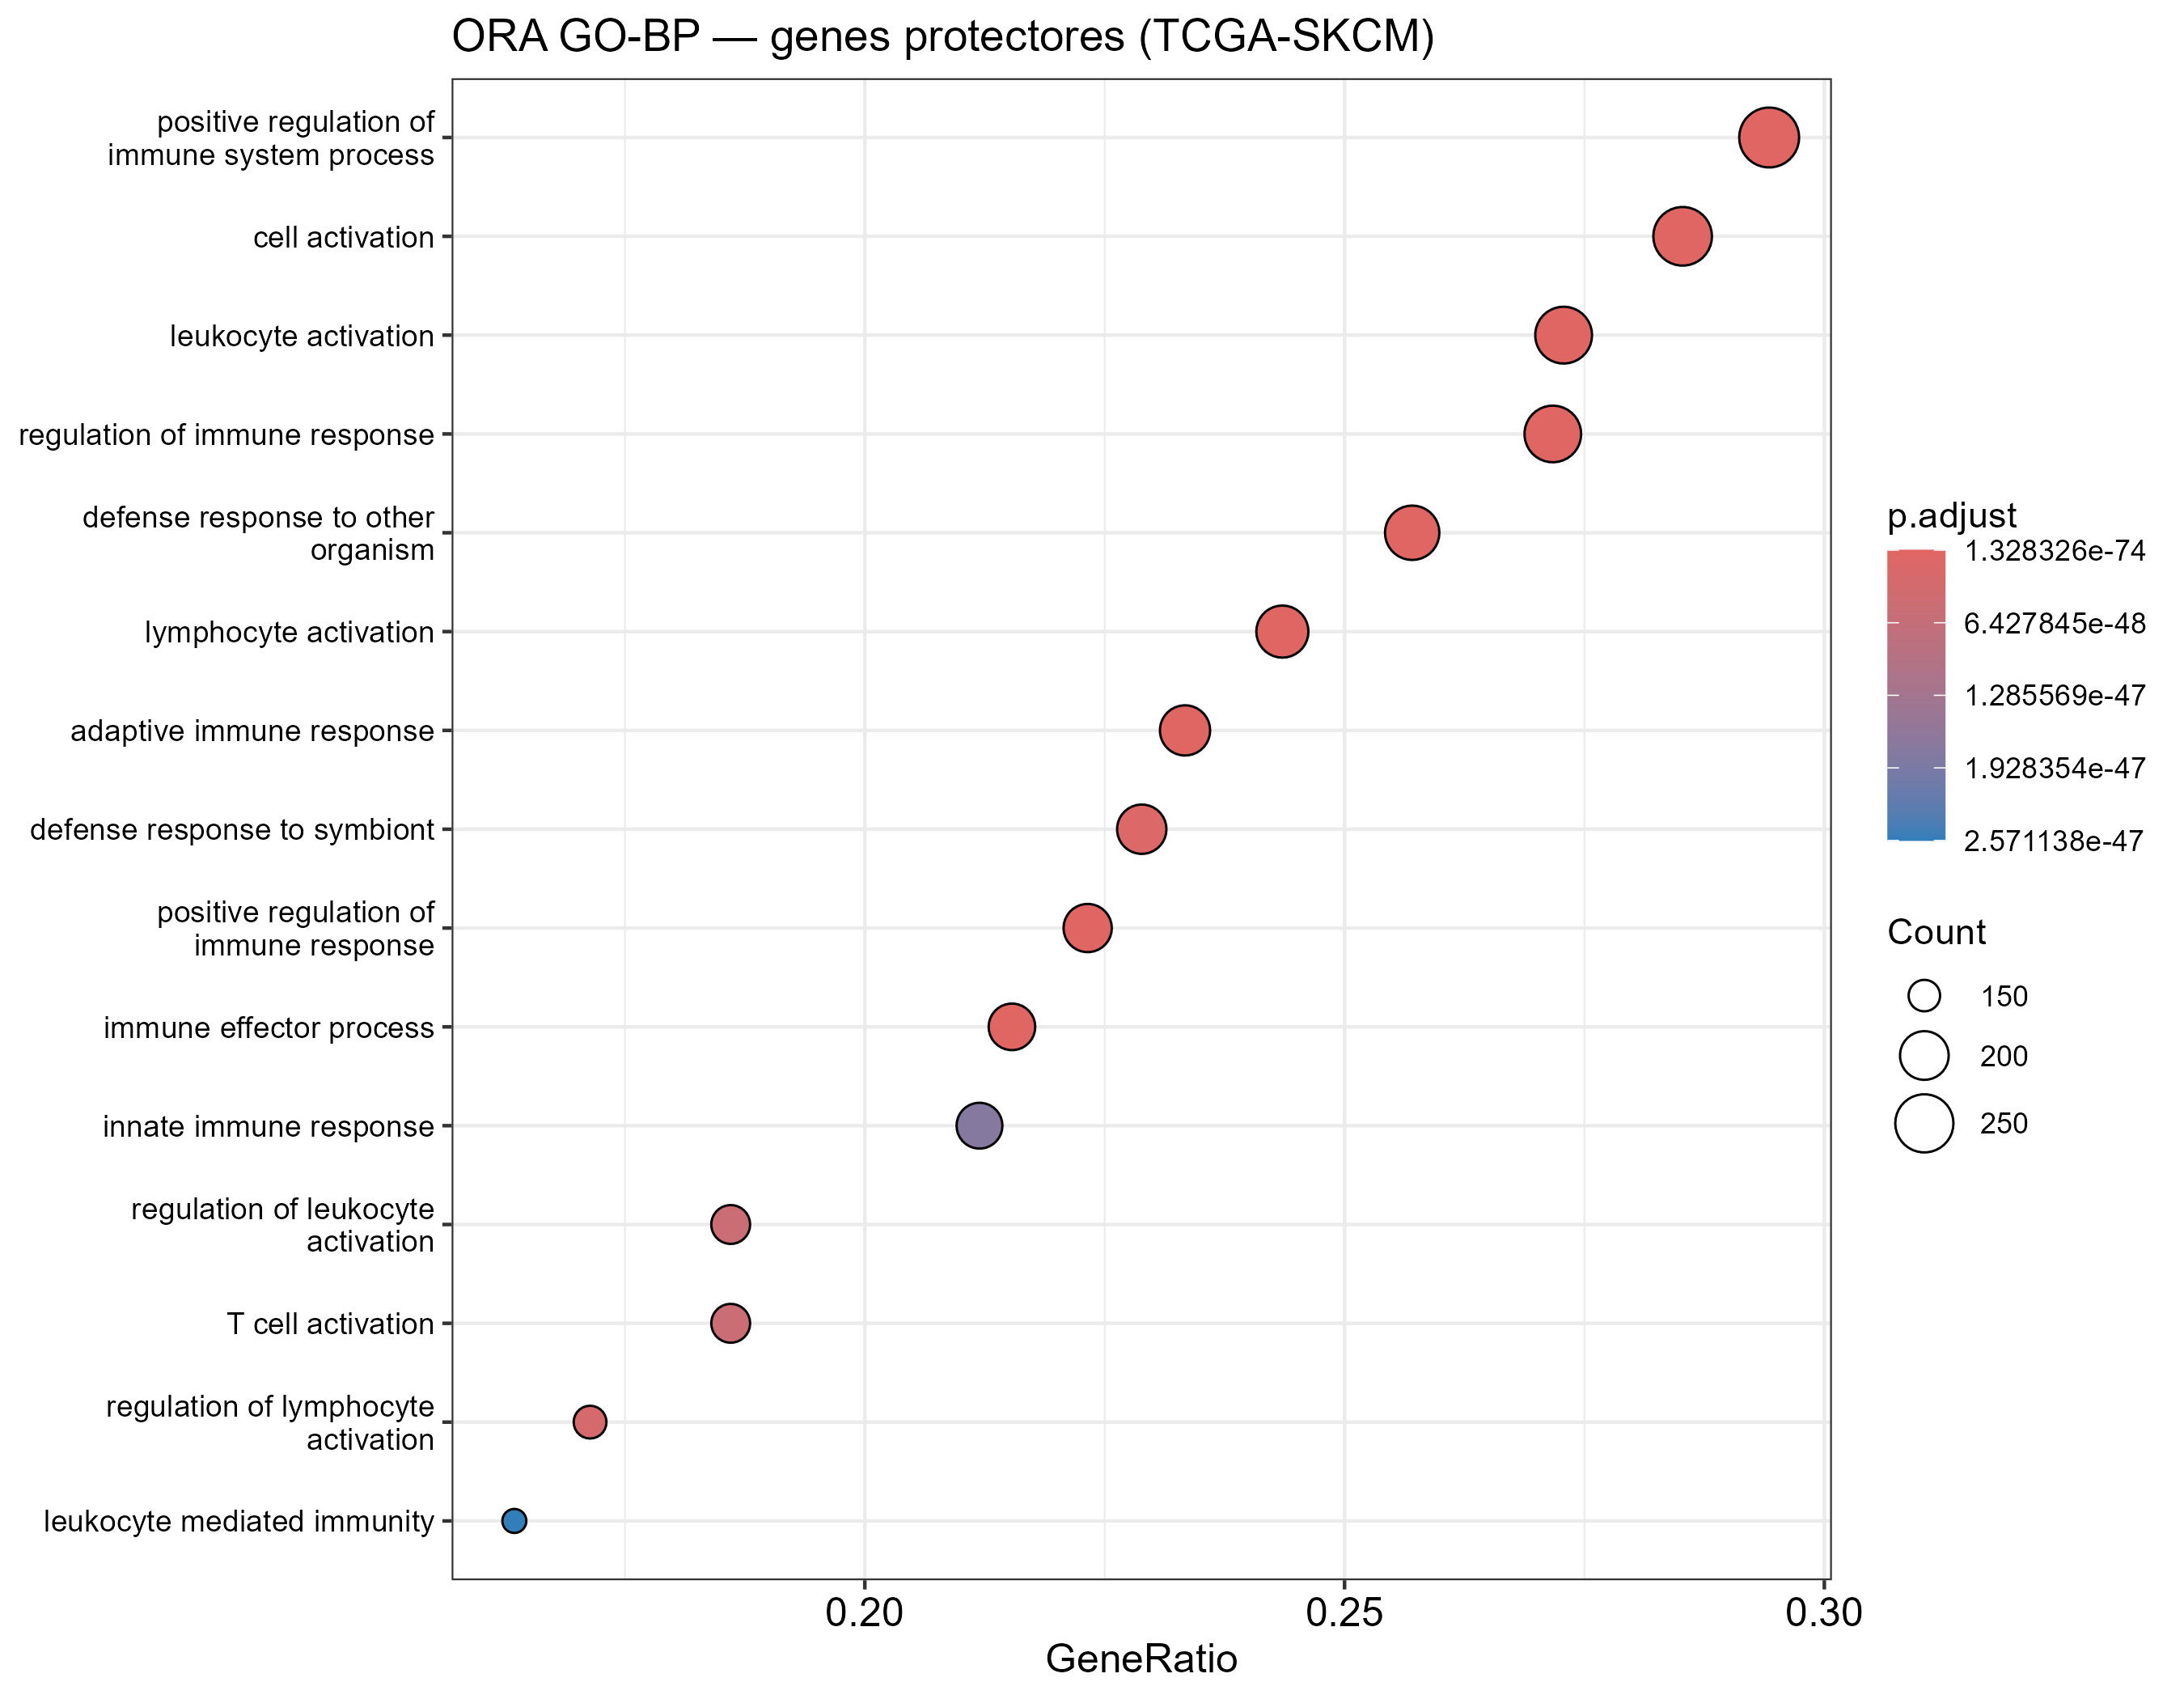
\includegraphics[width=0.90\textwidth]{figures/ora_go_protectores}
\caption{ORA GO-BP sobre los genes protectores del screening Cox (HR $< 1$, FDR $< 0{,}05$) en TCGA-SKCM. Cada punto representa un término GO-BP significativo; el tamaño indica el número de genes del conjunto de estudio que solapan con el término; el color indica el p-valor ajustado.}
\label{fig:ora_prot}
\end{figure}

\begin{figure}[H]
\centering
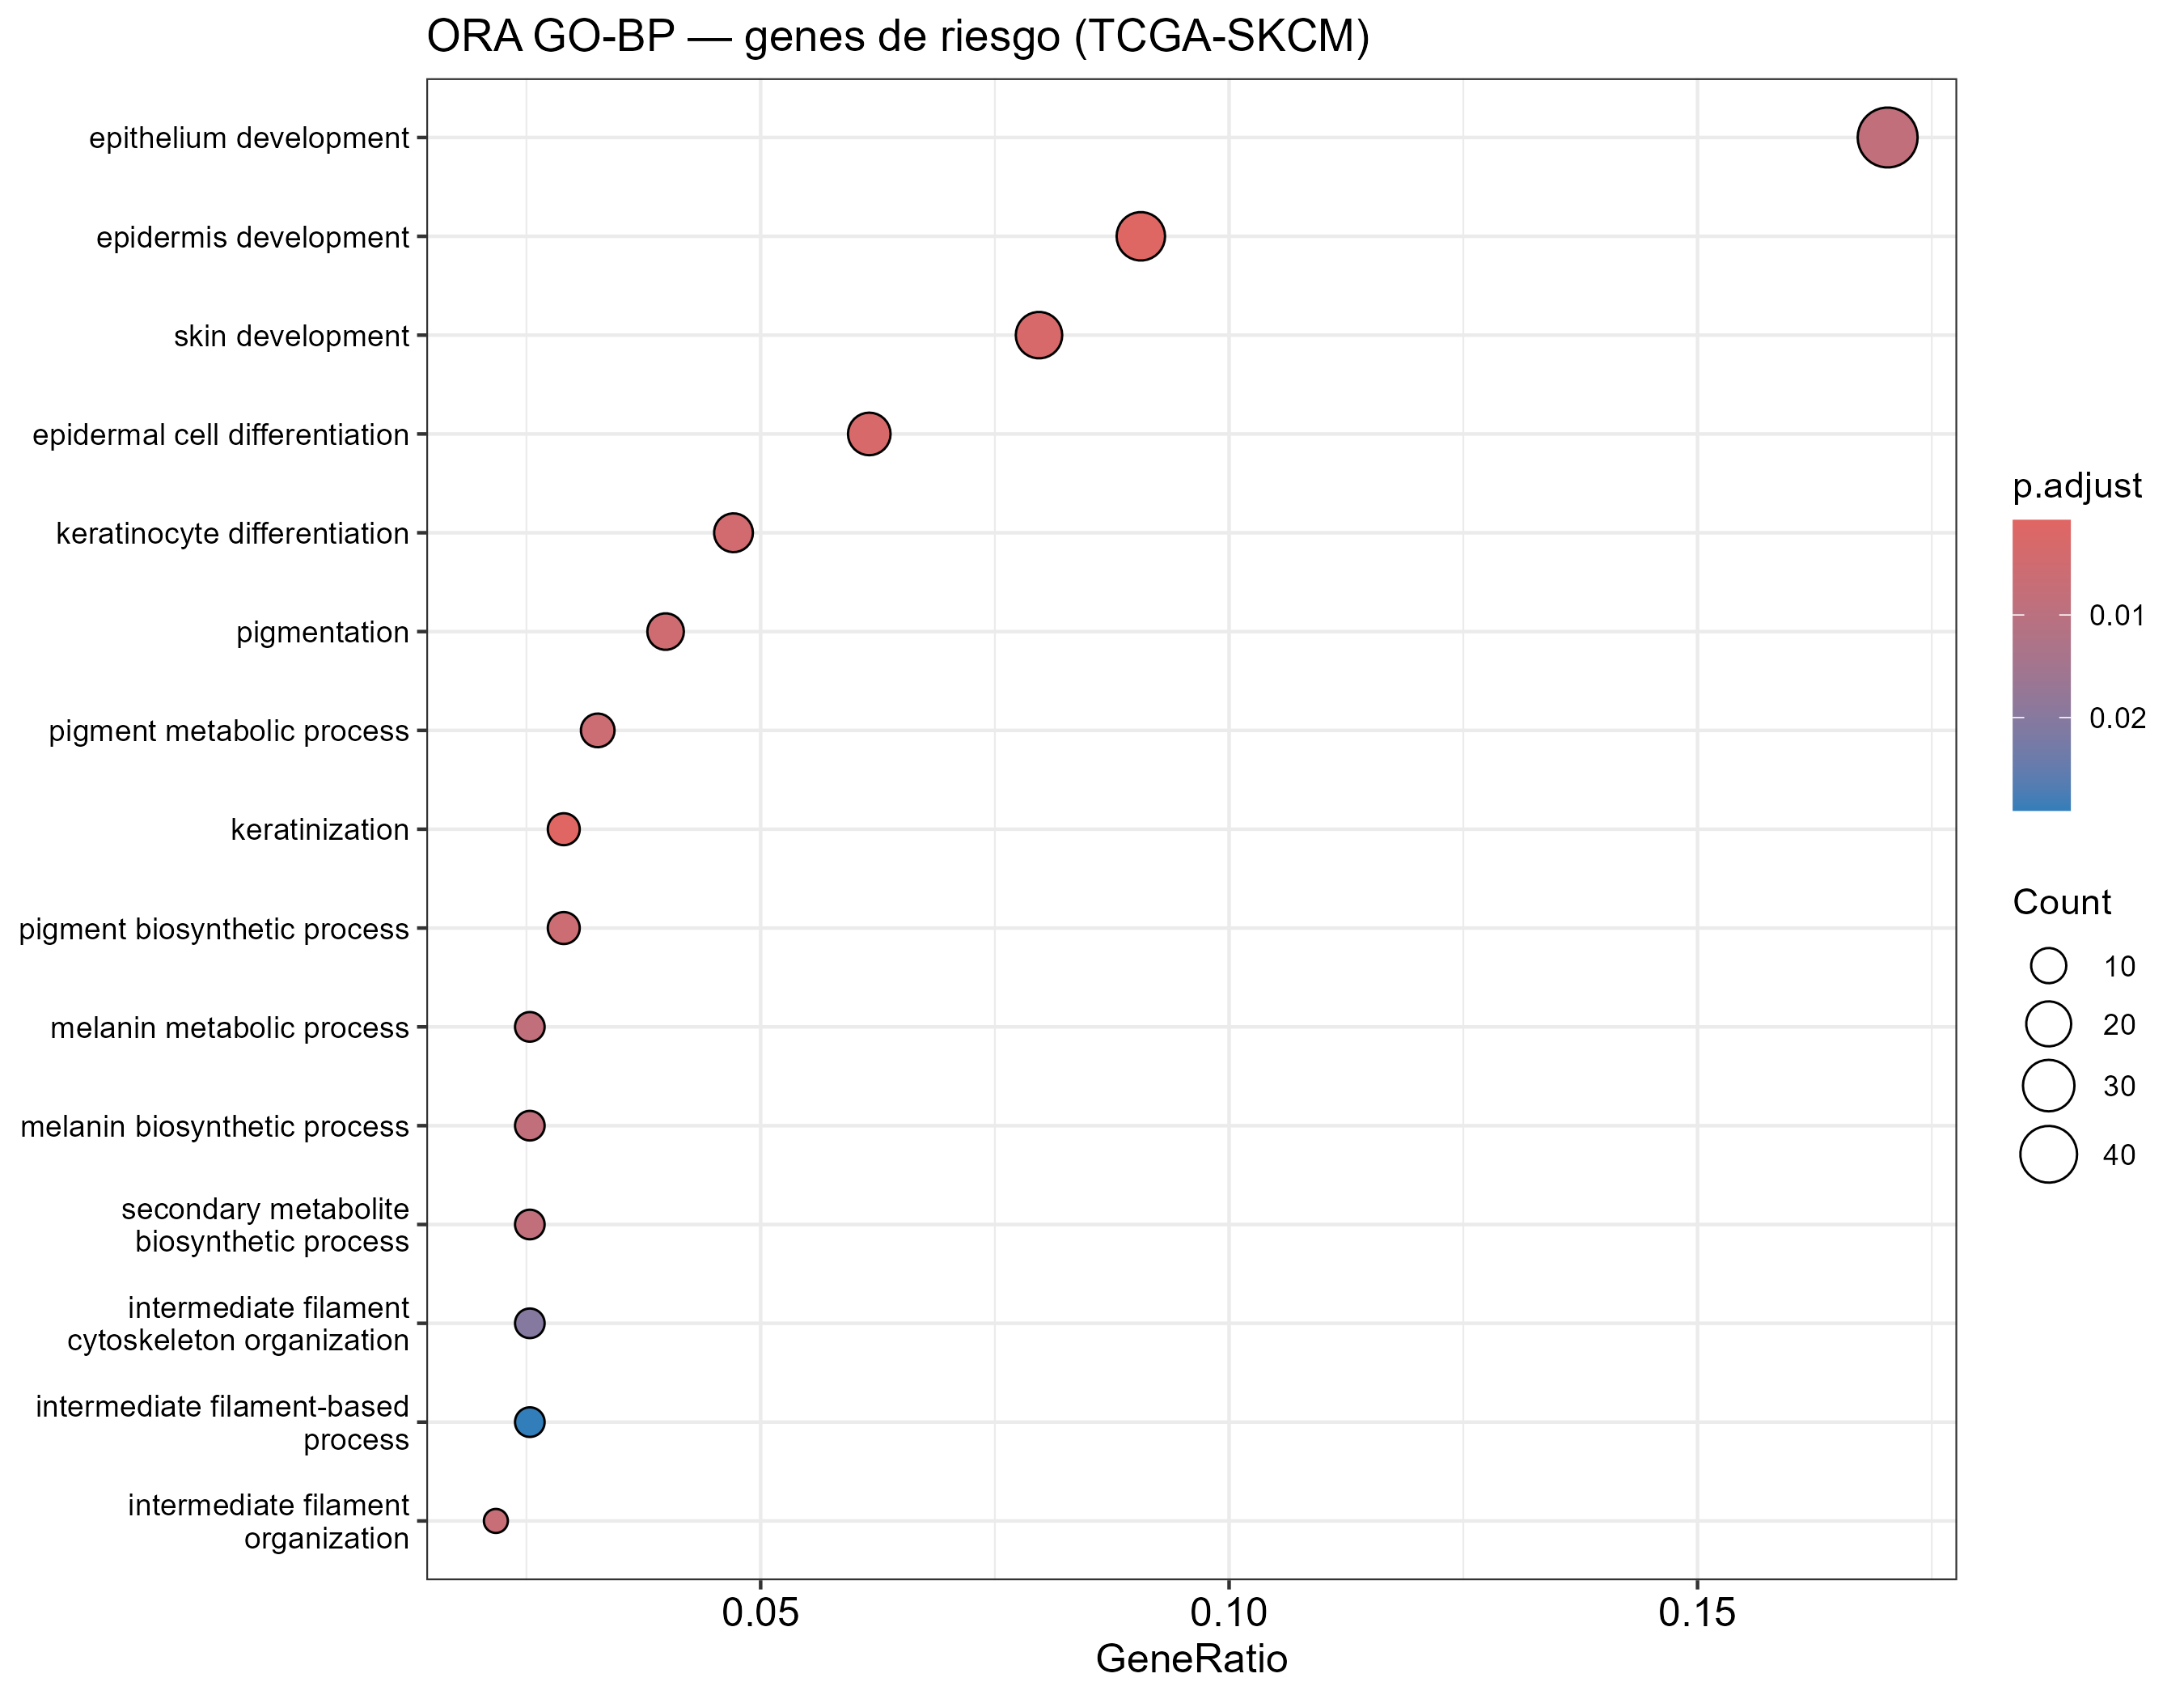
\includegraphics[width=0.90\textwidth]{figures/ora_go_riesgo}
\caption{ORA GO-BP sobre los genes de riesgo del screening Cox (HR $> 1$, FDR $< 0{,}05$) en TCGA-SKCM.}
\label{fig:ora_risk}
\end{figure}
